\section{Particle storage and vectorisation}
\label{section:vectorisation}

There are three different types of data sets in our minimalistic DEM codes: 
geometric data, behavioural data and meta data. 
Behavioural data is collision data.
It is modelled as struct with location and a normal vector.
Sets $\mathbb{C}$ of collision points are modelled as (dynamic) array of structs
(AoS) augmented with a copy of the collision partner as detailed before.
Spacetrees are our meta data.
The geometry data finally determines how straightforward and fast the collision
detection is. Collision detection is the computationally heavy activity in the
algorithm.
While other DEM discussions speak of a computational phase \cite{xxxx}, we
prefer activity, as the collision detections are split among the grid traversal
and interwoven with other activities.

\begin{figure}
 \begin{center}
  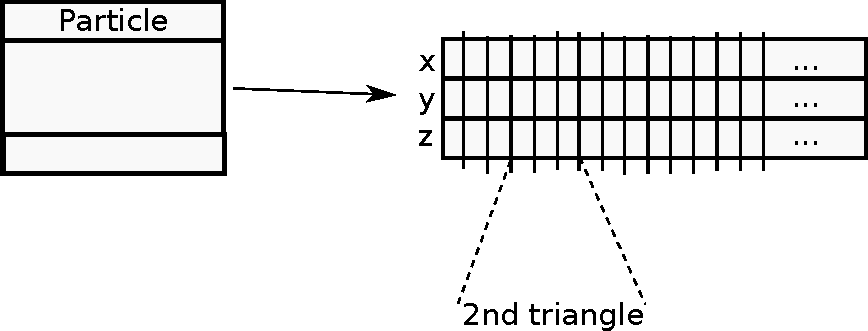
\includegraphics[width=0.5\textwidth]{sketches/data-structure.pdf}
 \end{center}
 \caption{
   Right: The two layer data layout of our DEM code with an AoS on the particle
   level but SoA for the vector entries with replicated vector entries.
 }
 \label{figure:data-structure}
\end{figure}

We propose to realise the geometric data in two layers (Figure
\ref{figure:data-structure}).
A hull struct holds all particle properties such as velocities, rotation, mass,
geometric centre and mass centre.
Vertices refer to these hulls with arrays of structures (AoS).
Hulls link with pointers to the actual geometric data. 
This data is realised as structure of array, i.e.~there is a sequence of
x-coordinates, a sequence of y-coordinates and a sequence of z-coordinates.
These sequences are blown up with redundant data.
The first three entries in the x array hold the x coordinates of the three
vertices of the first triangle of the particle mesh.
The entries four through six hold the coordinates of the second triangle and so
forth. 
The degree of redundancy is determined by the particle mesh.

We accept the increased memory consumption of such a structure but in return are
able to avoid any indirect addressing, process all geometry data in the
collision checks in a stream-like fashion and can align all vector entries. 
SoA data are notouriously difficult to handle if subsets of a dataset are to be
transferred or data is to be reordered.
In our particle handling, a particle is an atomic unity.
It is never teared apart or resorted during the simulation run.
A particle mesh is topologically invariant.

The remainder of this section discusses a function \texttt{findCollisions} that
is passed two particles or two particle meshes respectively and identifies all
contact points. 
Such an operation with quadratic complexity is often wrapped into an additional
check that compares bounding boxes and thus may skip comparisons
\cite{mattutis}.
We abstain from such a check as the spacetree realises a related optimisation.
The following text thus discusses a nested loop with the outer loop
running over all triangles in $\mathbb{T}_A$ and the inner loop running over all
triangles in $\mathbb{T}_B$. 

\subsection{Brute force geometric comparison}

\subsubsection{Segment to Segment Minimum Distance }
The calculation of the distance between segments [8,9] in three dimensions is a geometric calculation that involve getting the closest points by extending the line that they lie on until intersection, if the two lines intersect then the closest point on the two segments is on the boundaries of the segment.
The segment 
$$S1 = [P0, P1]$$
can be formulated as 
$$P(s) = P0+s(P1-P0) = P0+su$$
with a constraint on s, $0<=s<=1$. Similarly, the second segment 
$$S2 = [Q0, Q1]$$
is written as $$Q(t) = Q0+t(Q1-Q0) = Q0+tu$$ with constraint $0<=t<=1$. So, for $sC$ and $tC$ being the closest points on the corresponding extended segments lines L1 and L2, then if  both sC and tC are within the boundaries of the segments then the closest points are also the closest points on the respective segments. 
In the case where sC and tC correspond to points on L1 and L2 outside the range of either segment $S1$ and $S2$, then sC and tC do not also define the closest points on the segments $S1$ and $S2$. So it is necessary to determine points that minimize 
\begin{equation}
w(s,t) = P(s) - Q(t)
\end{equation}
over the ranges of the segments using the corresponding constraints. 
The problem can be formulated into a minimization problem where the equation w is the same as minimizing 
$$|w|^2 = w \cdot w= (P0+su-tv) \cdot (Q0+su-tv)$$

which is a quadratic function of s and t. The relation of $|w|^2$ define a parabolic equation over a (s,t)-plane (See Figure \ref{fig9}) with a minimum at $C = (sC, tC)$, it is strictly growing along the (s,t)-plane with starting point from C. But because segments $S1$ and $S2$ are concerned and not their respective extended lines $L1$ and $L2$, the required minimum region is not C but it is located over a subregion G of the (s,t)-plane. The global minimum at C may lie outside of G, however, in these cases, the minimum always occurs on the boundary of G, and in particular, on the part of G's boundary that is visible to C. That is, there is a line from C to the boundary point which is exterior to G, and it can be said that C can "see" points on this visible boundary of G (See Figure \ref{fig9}).

\begin{figure}[!h]
\centering
\includegraphics[width=0.3\textwidth]{sketches/ss_box} \protect\caption{\label{fig9}(s,t) parameter space with G boundary box C for global minimum}
\end{figure} 

Suppose that we want the minimum distance between two finite segments $S1$ and $S2$, then 
$$G=\{ (s,t) \: \| \: 0 \leq s \leq 1, 0 \leq t \leq 1 \} = [0,1]\times[0,1]$$ 
is a unit square in (s,t) space. The four edges of the square are given by point at $s = 0, s = 1, t = 0, t = 1$. If $C = (sC, tC)$ is outside the G area, then it can "see" at most two edges of G. If $sC < 0$, C can see the $s = 0$ edge, if $sC > 1$, C can see the s = 1 edge, and similarly for tC, so in this way there is an enforcement of the required constraints. When C is not in G, at minimum 1 and at maximum 2 of constraints are active, and they determine which edges of G are candidates for a minimum of $|w| ^2$.
 
For each candidate edge, to compute where the minimum that occurs on that edge, either in its interior or at an endpoint, it is possible to solve for the other unknown parameter since at minimum one is to be found (either t or s). So using the derivative of the $|w^2|$ equation it is always possible to solve for the parameter that is in the interior of G. For example when s = 0, $|w|^2 = ((P0-Q0)-tv) \cdot ((P0-Q0)-tv)$. Taking the derivative with $t$ it possible get a minimum when: $0 = \frac{d}{dt}|w|^2 = -2v \cdot ((P0-Q0)-tv)$.
This gives a minimum on an edge at (0, t0) where $t0 = \frac{(v \cdot (P0-Q0))}{(v \cdot v)}$
If $0 <= t0 < 1$, then this would be the minimum of $|w|^2$ on G, and P(0) and Q(t0) are the two closest points of the two segments. But in the case where t0 is outside G, then either (0,0) or (0,1), would be the minimum along that edge (since $s=0$). Using this method it is possible to perform only a couple of checks to find the minimum of w(s,t) that correspond to the minimum distance between the segments.

\subsubsection{Point to Triangle Minimum Distance}
The other calculation required by the naive approach is to perform the check of point to triangle distance[12, 10, 11]. This test complete the brute force approach since it doesn't leave any  space for cases where triangles are in a configuration where a point - triangle plane distance is the shortest distance in the initial triangle pair minimum distance problem. 

To understand the problem of computing the minimum distance between a point P and a triangle T, it is necessary to understand the parameterised coordinate system of triangles. A triangle can be described by its barycentric coordinates in a way that any point on it can be dependent on two parameters, such that 

$$T(s, t) = B + s \cdot E0 + t \cdot E1$$

where $B = point1$, $E0 = point2-point1$, $E1 = P3 - P1$ for 

$$(s,t) \in D = \{(s,t) : s \in [0,1],t \in [0,1],s + t ≤ 1\}$$ 

The minimum distance is computed by determining the values $(s, t) \in D$ in the squared-distance equation $Q(s, t) = |T(s, t) - P|^2$ where $T(s,t)$ correspond to a point on the triangle closest to P. The function is quadratic and can be written as: 
$$Q(s,t)=as^2 +2bst+ct^2 +2ds+2et+f$$

where $a = E0 \cdot E0$, $b = E0 \cdot E1$, $c = E1 \cdot E1$, $d = E0 \cdot (B - P)$, $e = E1 \cdot (B - P)$, and $f = (B - P) \cdot (B - P)$.

Quadratics are classified by the sign of $ac - b^2$ so for function Q, $ac - b2$ = $(E0 \cdot E0)(E1 \cdot E1) - (E0 \cdot E1)^2$ =$|E0 \cdot E1|^2 >0$. The positivity is based on the assumption that the two edges E0, E1 are linearly independent, so their cross product is a nonzero vector. Q is a continuously differentiable and the minimum occurs at an interior point of D where the gradient $Q = 2(as + bt + d, bs + ct + e) = (0, 0)$ or at a point on the boundary of D. The gradient of Q is zero only when 
$$s = (be - cd)/(ac - b^2)$$ and 
$$t = (bd - ae)/(ac - b^2).$$ 
If $(s,t) \in D$, then minimum of Q is found. For example considering that region 0 (See Figure \ref{fig10}) is the domain of Q, so $(s, t) \in D$. If (s, t) is in region 0, then the point on the triangle closest to P is interior to the triangle, not on its edge.

\begin{figure}[!h]
\centering
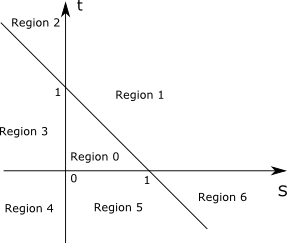
\includegraphics[width=0.4\textwidth]{sketches/pt_regions} \protect\caption{\label{fig10} Regions based on the (s,t) parameters plane}
\end{figure} 

On the other hand if the minimum is not in D then it should be should be on the boundary of the triangle and using the correct active constraints to restrict the solution using the region methodology. So if (s, t) is in region one then the elliptic level curves of Q are those curves in the s,t plane for which Q is constant. 

At the point where Q = (0,0), the level curve degenerates to a single point (s, t). The global minimum of Q occurs there ($V_{min}$). As the level values V increase from $V_{min}$, the corresponding levels are growing away from $(s,t)$. There is a smallest level value V0 for which the corresponding ellipse is tangent to the triangle domain $D$ edge $s+t = 1$ at a value $s = s0 \in [0,1], \: t0 = 1 - s0$. So for any level values $V < V0$, the corresponding ellipses do not intersect $D$. However for any portion of $D$ that intersect elliptic levels V must be $V > V0$. Therefore in this case point $(s0, t0)$ provides the minimum distance between P and the triangle where $t0$ is known $t0 = 1 - s0$ and $s0$ is the only unknown to be solved since the problem is decreased by one dimension. Moreover, when minimization is happening at $\nabla Q(s, 1 − s) = 0$ then there are three cases where $s > 1$ and $s$ has to be restricted to $s=1$ and the minimum occurs at $\nabla Q(1, 0)$ because of the barymetric triangle constraints, similarly if $s < 0$ then minimum occurs when $\nabla Q(0,1)$ or lastly $s \in [0,1]$ and has to be solved for a minimum at $\nabla Q(s,1-s)$.

Similarly the same technique for determining whether the minimum occurs at the endpoints or at the interior interval of the corresponding constraints, is performed for region three and region five (Figure \ref{fig10}). In the case where (s, t) occur in region three then the minimum has to occur at (0, t0) following the process like in region one where $t0 \in [0, 1]$. If $(s, t)$ is located in region five (Figure \ref{fig10}), then the minimum occurs at $(s0, 0)$ where $s0 \in [0, 1]$.  

When $(s, t)$ is located inside region two, there are three possibilities for the elliptic level curve that contact or intersect the boundaries of $D - region0$ area, the contact of the levels with the triangular region may occur in: 
\begin{enumerate}
\item edge where $s + t = 1$ 
\item edge where $s = 0$
\item at point where $t = 0$ and $s = 1$.
\end{enumerate}

That is because although the global minimum occurs in region two, there is a level curve of Q that contact the $D$ but the contact point and the region inside the level curve does not overlap. At these occurrences then the negative of the contacting level curve of Q cannot point inside $D$. For example for region two could be the direction of $-\nabla Q(0,1), -\nabla Q(s,1-t) and -\nabla Q(0,t),$ which points towards the inside of the level curve instead of inside $D$. 

In order to determine which of the three cases occur, it is possible to check which areas are negative so in a way it is possible to eliminate the cases where the contact doesn't occur and where it does. So if $\nabla Q = (Qs, Qt)$ and $Qs$ and $Qt$ are the partial derivatives of Q, it should be the case where $(0, -1) \cdot \nabla Q(0, 1)$ and $(1, -1) \cdot \nabla Q(0, 1)$ are not both  negative. The two vectors $(0, −1)$ and $(1, −1)$ are directions that correspond to the edges $s = 0$ and $s + t = 1$, respectively. The choice of edge $s+t = 1$ or $s = 0$ can be made based on the signs of $(0,-1) \cdot \nabla Q(0,1)$ and $(1, -1) \cdot \nabla Q(0, 1)$. Similarly as for region three, the same calculation technique is used for the regions four and six. 

\clearpage

\begin{algorithm}
 \caption{Brute-force distance calculation.} \label{algorithm:bf}
 \begin{algorithmic}[1]
	\Function{BF}{A, B, C, D, E, F}
	
		\State $T1=[A;B;C;];$
		
		\State $T2=[D;E;F;];$

		\State $list[0]= pt(T2, T1[0]);$

		\State $list[1]= pt(T2, T1[1]);$

		\State $list[2]= pt(T2, T1[2]);$

		\State $list[3]= pt(T1, T2[0]);$

		\State $list[4]= pt(T1, T2[1]);$

		\State $list[5]= pt(T1, T2[2]);$

		\State $ptmin = min(list);$

		\State $list[0]=segseg(T1[0],T1[1],T2(0],T2[1]);$

		\State $list[1]=segseg(T1[0],T1[1],T2[1],T2(2]);$

		\State $list[2]=segseg(T1[0],T1[1],T2[2],T2(0]);$

		\State $list[3]=segseg(T1[1],T1[2],T2[0],T2(1]);$

		\State $list[4]=segseg(T1[1],T1[2],T2[1],T2(2]);$

		\State $list[5]=segseg(T1[1],T1[2],T2[2],T2(0]);$

		\State $list[6]=segseg(T1[2],T1[0],T2[0],T2(1]);$

		\State $list[7]=segseg(T1[2],T1[0],T2[1],T2(2]);$

		\State $list[8]=segseg(T1[2],T1[0],T2[2],T2(0]);$

		\State $ssmin = min(list);$

		\State $min = min(ssmin, ptmin);$

		\State $P = min.p; Q = min.q;$
	\EndFunction
 \end{algorithmic}
\end{algorithm} 


\begin{algorithm}
 \caption{Point to triangle distance algorithm.} \label{algorithm:bf}
 \begin{algorithmic}[1]
	\Function{pt}{T, Point}
		
		%function to evaluate Q(s,t) of triangle T 		
		
		\If{PointProjection in Region 0}
		
			\State {evaluate value of Q}
		
		\EndIf		
		
		\If {PointProjection in Region 1}
		
			\State {determine (s,t) parametric space values}
		
		\EndIf
			
		\If {PointProjection in Region 2}

			\State {determine (s,t) parametric space values}

		\EndIf			
		
		\If {PointProjection in Region 3}
		
			\State {determine (s,t) parametric space values}

		\EndIf
						
		\If {PointProjection in Region 4}
		
			\State {determine (s,t) parametric space values}
		
		\EndIf
				
		\If {PointProjection in Region 5}		

			\State {determine (s,t) parametric space values}

		\EndIf
				
		\If {PointProjection in Region 6}	

			\State {determine (s,t) parametric space values}
			
		\EndIf		
		
		\Return $Q point on triangle$
	\EndFunction
 \end{algorithmic}
\end{algorithm} 

\begin{algorithm}
 \caption{Segment to segment distance algorithm.} \label{algorithm:bf}
 \begin{algorithmic}[1]
	\Function{pt}{segment1, segment2}
		
		%function to evaluate (s,t) of seg1, seg2
		\If {segment1 and segment2 are parallel}		
		
			\Return {any point P on segment1 and any point Q on segment2}
		
		\Else 
			
			\State {Get the closest points sC and tC on the infinite lines L1, L2}
			
			\If {sC < 0, the s = 0 edge is visible}
				
				\State {s = 0}
				
			\EndIf
				
			\If {sC > 0, the s = 1 edge is visible}

				\State {s = 1}			
				
			\EndIf
				
			\If {tC < 0, the t = 0 edge is visible}

				\State {t = 0}

			\EndIf
								
			\If {tC > 0, the t = 1 edge is visible}

				\State { t = 1}

			\EndIf							
		\EndIf
		
		\Return {P, Q points on two segments}
		
	\EndFunction
 \end{algorithmic}
\end{algorithm} 

%
% How does the algorithm work. Robustness
%
Our default brute force approach implementation runs per triangle pair through all possible distance
configurations (Algorithm \ref{algorithm:bf}).
First, we run through all six involved vertices and compute the distance to the
other triangle.
Second, we determine the distances between each line segment-to-line segment combination.
This yields 9+6=15 comparisons in total.
The minimum distance results from a minimum over all computed distances.
It is a robust approach, it always yields the correct answer.


%
% Speed, character
%
The algorithm is \ldots 

A fusion of multiple steps is not possible since all parametric/geometric scenarios have to be evaluated separately and naively. As shown the algorithm in Figure (x) the geometric checks and the brute force character of the algorithm does not allow computational fusion of execution branching. 




\subsection{Penalty-based formalism}

The second approach to solve the triangle-to-triangle  distance problem by parameterisation of the triangles such that the distance between them is formulated as a quadratic function. The approach is an iterative solution and it is approximated with the Newton method.

The method rely on the optimization-based formulation of the distance between two points. Let $x$ and $y$ be two points, belonging respectively to triangle $T_1$ and $T_2$. Assuming that points $A, B, C$ are vertices of $T_1$ and that points $D, E, F$ are vertices of $T_2$, $x$ and $y$ can be defined using the following equations: 
\begin{align*}
T_{1}:x(a,b)=A+(B-A) \cdot a+(C-A)\cdot b
\end{align*}
\begin{align*}
T_{2}:y(g,d)=D+(E-D) \cdot g+(F-D) \cdot d
\end{align*} 
To find the minimum distance between $T_1$ and $T_2$ and the corresponding two closest points $P$, $Q$ on the two triangles we minimize
\begin{align*}
f\left(a,b,c,d\right)=\left\Vert x\left(a,b\right)-y\left(c,d\right)\right\Vert ^{2}
\end{align*} 

What has to be noted is that $x$ and $y$ have to stay within the area of the two triangles. The four parameters of the function $f$ have to comply with six inequality constraints:
\begin{align*}
min_{a,b,g,d} f(a,b,g,d)
\end{align*}  
$$such \:that: \: \{a\geq0,b\geq0, a+b\leq1, d\geq0, g\geq0, g+d\leq1 \}$$ 


\begin{figure}[htb]
  \begin{center}
    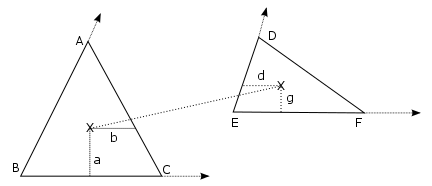
\includegraphics[width=0.6\textwidth]{sketches/c.png}
  \end{center}
  \caption{
    Example of minimum distance and the corresponding barycentric points (parameters of objective function) on a pair of triangles in 3D. Triangle X:T1 has points A, B, C where barymetric parameters a,b correspond to point $x$ on the triangle. Triangle Y:T2 has points D,E,F where barymetric parameters g,d correspond to a point $x$. The two defined barymetric points define the minimum distance between the two triangles in 3D.
  }
  \label{figure:barycentric_contact}
\end{figure}

To enforce the constraints the problem is transformed into a series of unconstrained problems with the augmentation of the objective function $f$ using the penalty-based method. The penalty function penalizes the iteration so that the boundaries of the feasible region are valid. Although there are factors that determine the number of iterations required the tuned-to-the-problem parameters yield a good number of Newton iterations that cannot be reduced to less than two; (initial guess to penalized boundary step, correction step).

\begin{figure}[htb]
  \begin{center}
    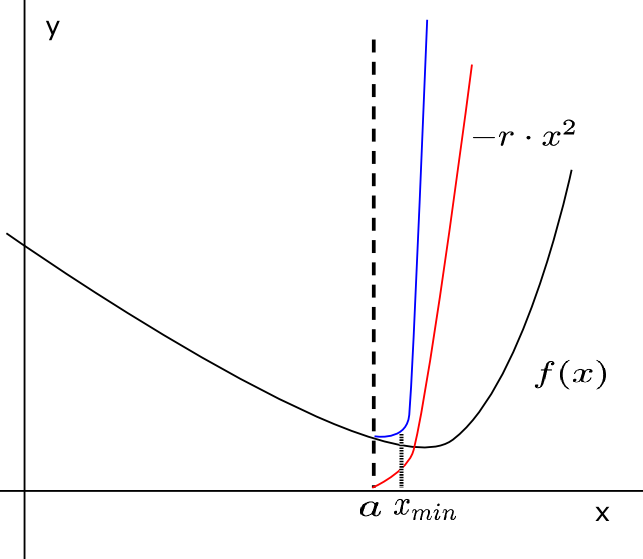
\includegraphics[width=0.5\textwidth]{sketches/penalty.png}
  \end{center}
  \caption{
Illustration of a 2D problem showing the penalty function (red line) penalizing the objective function (black line) f(x) under a constraint $a$ (dash line) to create the feasible region (blue line).
  }
  \label{figure:penaltyfunction}
\end{figure}

This approach adds a penalty term to the objective function to penalize the solution when outside of the feasible region: 
\begin{equation}\label{eq:penalty}
P(x)=f(x)+r\sum_{i=1...6}max(0,c(x_{i}))^{2}
\end{equation}
Where r is the penalty parameter (Figure \ref{}). Newton iterations always converge to a solution slightly on the outside of the feasible region. Convergence can be controlled by the r parameter that controls the sharpness of the curve for the constraints. One aspect that requires care however is the invertibility of the Hessian $\nabla\nabla P$. 

Furthermore the problem is ill conditioned and a Quasi-Newton method is used. The Hessian matrix is not invertible so it is not possible to solve the direction of the search by computing the Hessian and gradient. This illustrates the fact that $f$ has multiple minima and $\nabla\nabla f$ is singular. Consequently, $\nabla\nabla P$ is also singular inside of the feasible region. The ill conditioning is caused by the problem definition itself, where there is a state where there are multiple solutions to the problem based on the orientation of the two triangles. This is also revealed by the two zero eigenvalues of the Hessian. Because of the ill-conditioning, we use a quasi-Newton approach, where the Hessian is approximated by a perturbed operator $\nabla\nabla P + \epsilon I$. $I$ is an identity matrix and $\epsilon$ is suitably small.

\begin{algorithm}
	\protect\caption{\label{alg4}Penalty Solver.}
	\begin{algorithmic}[1]
	
	\Function{Penalty}{A, B, C, D, E, F, rho, tol}

		\State $BA~=~B-A;~CA~=~C-A;~ED~=~E-D;~FD~=~F-D;$

		\State $hf~=~{[}2{*}BA{*}BA',~2{*}CA{*}BA',-2{*}ED{*}BA',-2{*}FD{*}BA';$

		\State $2{*}BA{*}CA',~2{*}CA{*}CA',-2{*}ED{*}CA',-2{*}FD{*}CA';$

		\State $2{*}BA{*}ED',-2{*}CA{*}ED',~2{*}ED{*}ED',~2{*}FD{*}ED';$

		\State $2{*}BA{*}FD',-2{*}CA{*}FD',~2{*}ED{*}FD',~2{*}FD{*}FD'{]};$

		\State $x~=~{[}0.33;~0.33;~0.33;~0.33{]};$

		\For{i=1:99}

			\State $X~=~A+BA{*}x(1)~+~CA{*}x(2);$

			\State $Y~=~D+ED{*}x(3)~+~FD{*}x(4);$

			\State $gf~=~{[}2{*}(X-Y){*}BA';~2{*}(X-Y){*}CA';~-2{*}(X-Y){*}ED';~-2{*}(X-Y){*}FD'{]};$

			\State $h~=~{[}-x(1);~-x(2);~x(1)+x(2)-1;~-x(3);~-x(4);~x(3)+x(4)-1{]};$

			\State $dh~=~{[}-1,~0,~1,~0,~0,~0;~0,~-1,~1,~0,~0,~0;$

			\State $0,~0,~0,~-1,~0,~1;~0,~0,~0,~0,~-1,~1{]};$

			\State $mask~=~h'~$>$=~0;$

			\State $dmax~=~dh.{*}~{[}mask;~mask;~mask;~mask{]};$

			\State $gra~=~gf~+~rho~{*}~dmax~{*}~max(0,h(:));$

			\State $hes~=~hf~+~rho{*}dmax{*}dmax'~+~eye(4,4)/rho^2;$

			\State $dx~=~hes\textbackslash{}gra;$

			\State $DX~=~BA{*}dx(1)~+~CA{*}dx(2);$

			\State $DY~=~ED{*}dx(3)~+~FD{*}dx(4);$

			\State $error~=~sqrt(DX{*}DX'+DY{*}DY');$

			\If{error~$<$~tol}
				\State $BREAK;$
			\EndIf

			\State $x~=~x~-~dx;$

		\EndFor

	\EndFunction
	\end{algorithmic}

\end{algorithm}


The penalty algorithm as shown in Algorithm \ref{} accepts A, B, C, D, E, F vector coordinates for triangle T1(A, B, C), T2(D, E, F) as well as the required parameters for the algorithm to be solved. Rho is the penalty parameter that controls the steepness of the P(x) function (equation \ref{eq:penalty}) , eps is the perturbation parameter for the hessian matrix of the problem along its diagonal to make the matrix solvable. Tol is the tolerance for convergence (Floating point accuracy). In line 23 of Algorithm \ref{} an initial guess is chosen to be the center of the two triangles, then the for loop initiates the Newton iterations to find the points on the X, Y triangle planes under the constraints c. For each of the six constraints (line 12) the max function of the penalty is determined so that every possible active constraint is detected. In line 17 and line 18 the gradient and Hessian of P Penalty function is evaluated to be provided to the Gaussian elimination direct solver so that a Newton direction DX is solved. If the Newton step is large enough over the specified tolerance then the iteration is converged else the direction is used and the loop is executed once more recursively.

The penalty method is well-suited for SIMD optimisation because we can concurrently determine the distance between multiple triangle pairs as long as we use the same number of Newton steps: Up to four or eight
triangle pair distances can be determined at the same time; depending on the vector width. Such a speed-up statement however has to be read carefully. While the concurrency is high, it is not clear a priori how many Newton steps are required. A high number of Newton steps can render the penalty method slower than the brute force approach.
\subsection{Hybrid approach}
To create a hybrid solver we first assume that on average there are for each triangle pair distance computation only a few iterations that are required to arrive to a solution \ref{}. Based on empirical studies and tuning of the penalty parameter and the regularization variable, the majority of triangle pairs are solved within four iterations as shown in Figure {}. Secondly we set a user defined tolerance of error to the method to act as the switching point for the falling-back to brute force solver. If the number of fall backs does not overtake the number of penalty-based solutions then the method is a compromise between brute force and penalty both in terms of performance but also in terms of error of solution. 

\begin{figure}[htb]
  \begin{center}
    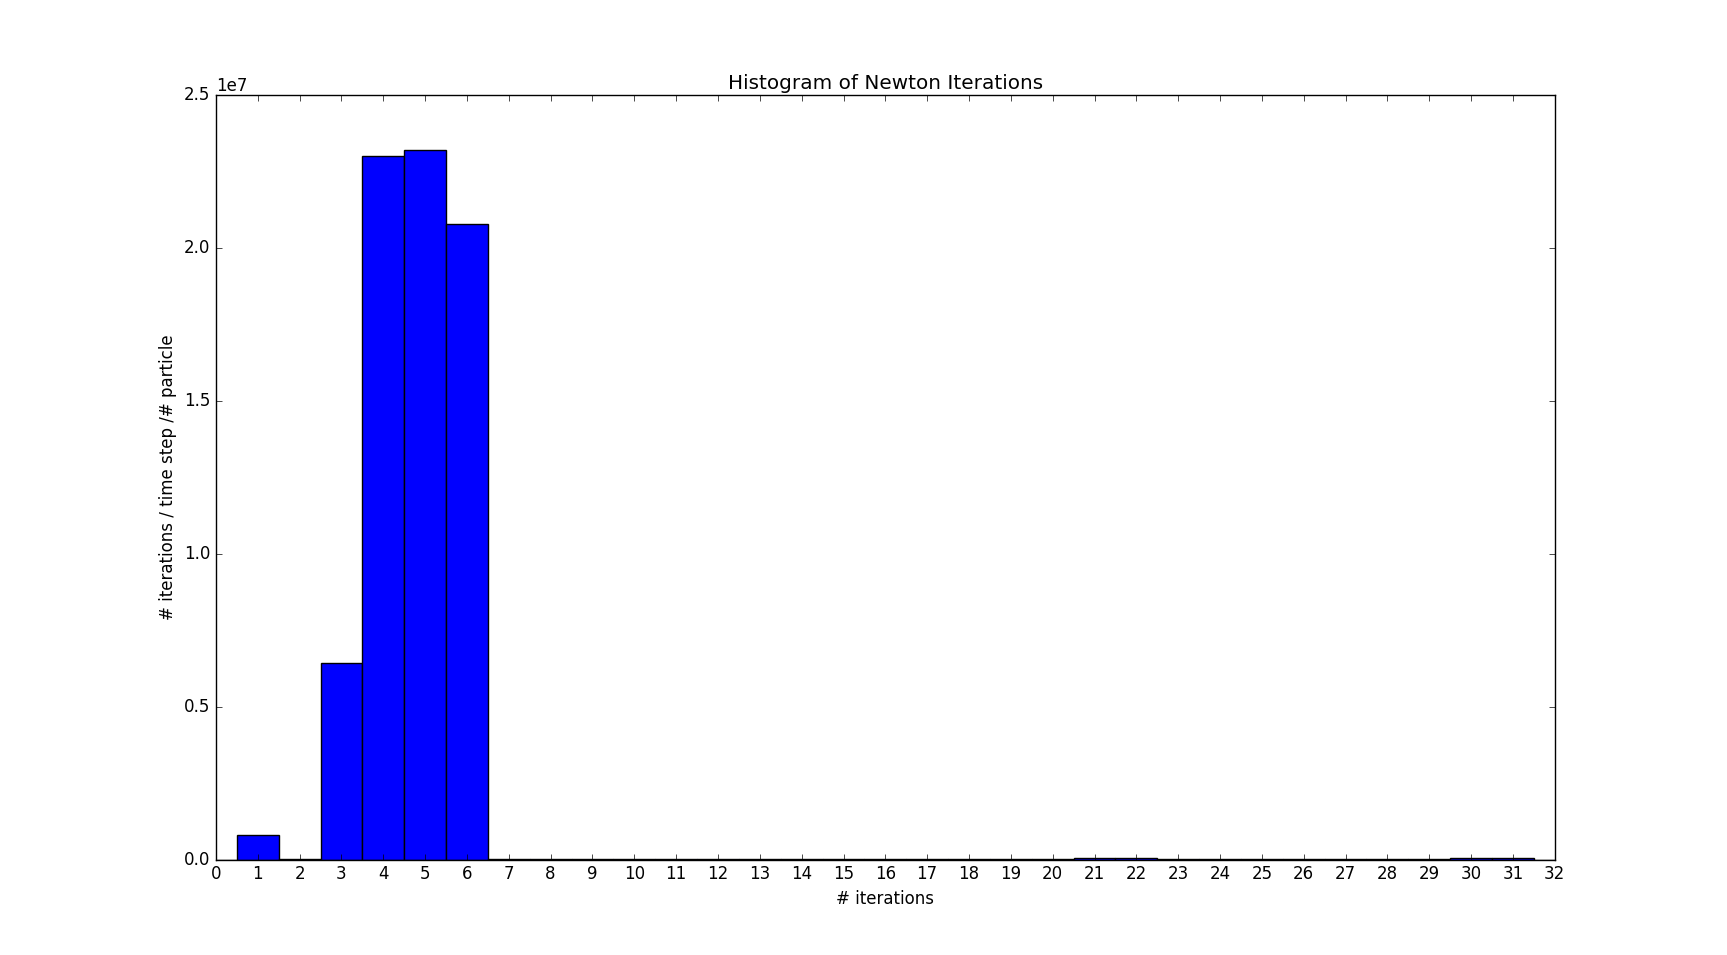
\includegraphics[width=1\textwidth]{experiments/random/penalty-stats/bar.png}
  \end{center}
  \caption{Histogram of number of iterations required by Newton Method for convergence on a sample of twenty four million triangle pair configurations.}
  \label{figure:newton_hist}
\end{figure}

There are two variants of hybrid method; the first is the hybrid-on-triangle-pairs and the second one is hybrid-on-triangle-batches. Both variants are developed to exploit the robustness of brute force while keeping the arithmetic intensity of the penalty method. The implementation of both methods takes into account the potential for shared memory scaling as well as data access continuity. In addition SIMD vectorised performance of the underlying methods and memory alignment are critical for the execution of both methods.

The first variant is hybrid-on-triangle-pairs where it divides the computational workload to be per each triangle pair. The hybrid-on-triangle-pairs method runs first the penalty solver on one triangle pair, if the solution is not within the user specified tolerance, we fall back to brute force to solve the problem naively. 

\begin{algorithm}
 \caption{Hybrid On Triangle Pairs} \label{algorithm:hybridTriangle}
 \begin{algorithmic}[1]

	\Function {hybridOnTrianglePairs(particleA, particleB, tolerance)}	
	
		\For {i = 0 to n particleA.triangles}
	
			\For {j = 0 to n particleB.triangles}
			
				\State {triangleError = penalty(particleA[i], particleB[j])}

				\If {triangleError > tolerance}

					\State {bruteForce(particleA[i], particleB[j])}
	
				\EndIf
	
			\EndFor
			
		\EndFor
		
		\Return {P, Q points on two triangles}
	
	\EndFunction
	
 \end{algorithmic}
\end{algorithm} 

The other variant is the hybrid-on-batches where it is hybrid per triangle batches. This method is checking the error less frequently than the previous variant and uses an error for the whole batch. As in the hybrid-on-triangle-pairs variant; we run then penalty method on one batch of triangles and then fall back to brute on the whole batch if the error tolerance is not satisfied. The batch size can be set by the user to be of any arbitrary size. For our application we set it to be the number of triangles of our non-spherical particles (tessellation size of 60~ triangles).    

\begin{algorithm}
 \caption{Hybrid On Triangle Batches} \label{algorithm:hybridBatches}
 \begin{algorithmic}[1]
	
	\Function {hybridOnTrianglePairs(particleA, particleB, tolerance)}	
	
		\For {i = 0 to n particleA.triangles}
	
			\For {j = 0 to n particleB.triangles (batchSize)}
					
				\State {batchError = penalty(particleA[i], particleB[j])}

			\EndFor
			
			\If {batchError > tolerance}
				
				\For {j = 0 to n particleB.triangles}
	
					\State {bruteForce(particleA[i], particleB[j])}

				\EndFor
	
			\EndIf
	
		\EndFor
	
		\Return {P, Q points on two triangles}	
	
	\EndFunction
	
 \end{algorithmic}
\end{algorithm} 

Both hybrid methods suffer by their nature by the granularity of the grain size whether that is singular size (triangle pair) or greater (batches of pairs).
The memory distribution of pairs of triangles that do not converge within the mean number of Newton iterations are not known a priori because the solution depends on the underlying geometry. Triangle pairs or triangle batches that do not converge within the set tolerance skew the overall error distribution margin, potentially creating the worse case scenario where the method becomes a worse than brute force solver with both penalty and brute force being executed in sequence. It is not possible to predict the sparsity/distribution of non-convergent triangle pairs/batches during run-time so the tolerance value, penalty, regularization parameters are vital. In our experiments those parameters are set based on empirical tuning and trial and error.


